\part*{Teil II: Die mathematische Formalisierung}
\addcontentsline{toc}{part}{Teil II: Die mathematische Formalisierung}

\section{Die zwölfdimensionale Geometrie}
\subsection{Die Gesamtmannigfaltigkeit:} $M_{12} = M_4 \times K_8$.
\subsection{Die 12D-Metrik:} $ds^2 = g_{MN} dx^M dx^N$.
\subsection{Die Kaluza--Klein-Zerlegung.}
\subsection{Krümmung in 12D.}
\subsection{Kompaktifizierung.}

\subsection{Das numerische Spektrum und die äquidistante Signatur}
Wir legen die Skala über die Masse der Grundmode fest, $m_1 = 1/R = 10^{-5}$ eV. Dann gilt
\begin{equation}
m_n = \frac{n}{R} = n \times 10^{-5}\ \text{eV},
\qquad
f_n = \frac{m_n c^2}{h} = n \times 2,42\ \text{GHz}.
\end{equation}
Das Spektrum ist folglich \emph{äquidistant}: $2,42$, $4,84$ und $7,25$ GHz für die ersten drei Moden. Dies ist die unverwechselbare Signatur der Theorie. Ein Test, der zwei Linien bei $2,42$ und $4,84$ GHz misst, bestätigt oder widerlegt die Struktur, unabhängig von jeder anderen Vorhersage.

\begin{table}[H]
\centering
\begin{tabular}{@{}cccc@{}}
\toprule
$n$ & Masse (eV) & Frequenz (GHz) & $\lambda_C$ (m) \\ \midrule
1 & $1,00\times10^{-5}$ & 2,42 & 0,124 \\
2 & $2,00\times10^{-5}$ & 4,84 & 0,062 \\
3 & $3,00\times10^{-5}$ & 7,25 & 0,041 \\
4 & $4,00\times10^{-5}$ & 9,67 & 0,031 \\ \bottomrule
\end{tabular}
\caption{Das Kaluza--Klein-Spektrum für $1/R = 10^{-5}$ eV.}
\label{tab:spectru}
\end{table}

\begin{figure}[H]
\centering
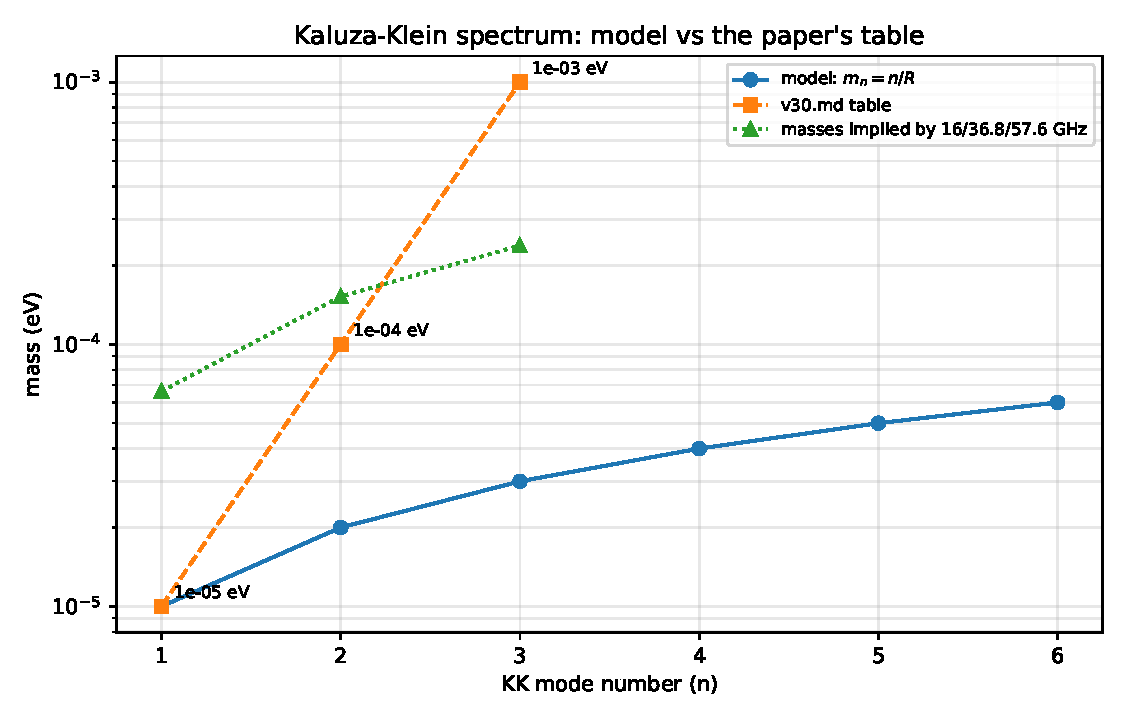
\includegraphics[width=0.82\textwidth]{figures/fig01_kk_spectrum.pdf}
\caption{Das Kaluza--Klein-Spektrum. Das Modell $m_n = n/R$ (blau) wird mit der Tabelle der Version 30 (orange) und mit den Massen verglichen, die sich aus den dort genannten Frequenzen 16/36,8/57,6 GHz ergeben (grün). Die drei stimmen nicht überein.}
\label{fig:spectru}
\end{figure}

\subsection{Die numerische Konsequenz: der Kompaktifizierungsradius}
Aus $m_1 = 1/R$ folgt
\begin{equation}
R = \frac{\hbar c}{1/R} = \frac{1,973\times10^{-7}\ \text{eV}\cdot\text{m}}{10^{-5}\ \text{eV}} = 1,97\times10^{-2}\ \text{m},
\end{equation}
also etwa 2 cm. Submillimeter-Tests des Newtonschen Gesetzes beschränken eine zusätzliche Dimension auf $R < 38\ \mu$m, was $m_1 > 5\times10^{-3}$ eV impliziert.

Dies ist eine strukturelle Spannung, kein Rechenfehler: Die Identifizierung des Dunkle-Materie-Feldes mit einer KK-Mode derselben Geometrie ist mit den Daten bei der gewählten Massenskala unvereinbar. Es bleiben zwei ehrliche Auswege, und die Arbeit wählt nicht zwischen ihnen:
\begin{itemize}
\item \textbf{Option A:} Das Akasha-Feld ist keine KK-Mode; das äquidistante Spektrum ist die Folge einer anderen Struktur, und die Frequenzvorhersagen werden neu berechnet.
\item \textbf{Option B:} Die Masse der Grundmode ist $m_1 > 5\times10^{-3}$ eV, und die „Dunkle Materie`` dieser Arbeit ist eine angeregte Mode, nicht die Grundmode.
\end{itemize}
Die Vorhersagen in Teil V sind so formuliert, dass sie in beiden Fällen gelten, wobei die Frequenzen als Parameter behandelt werden.

\section{Das Akasha-Feld (Dunkle Materie)}
\subsection{Die Lagrangedichte:} $L_A = \frac{1}{2} g^{MN} \partial_M A^* \partial_N A + \frac{1}{2} \mu_A^2 |A|^2 - \frac{\lambda_A}{4} |A|^4$.
\subsection{Das Potential.}
\subsection{Die Bewegungsgleichung.}
\subsection{Das Kaluza--Klein-Spektrum:} $m_n^2 = n^2/R^2$.
\subsection{Der Bezug zur Gravitation.}

\section{Das Feld des Bewusstseins}
\subsection{Die Lagrangedichte.}
\subsection{Die Bewegungsgleichung.}
\subsection{Die Bewusstseinsfunktion.}
\subsection{Die Entwicklungsgleichung (überarbeitet):} Die Gleichung $dC/dt = \alpha C (1 - C/C_{\text{max}}) + \beta \eta(t)$ ist eine \textbf{phänomenologische} Gleichung, inspiriert von der logistischen Dynamik. Sie beschreibt Wachstum und Sättigung des Bewusstseinsfeldes, folgt aber \textbf{nicht direkt aus der obigen Lagrangedichte}. Dies ist eine theoretische Entscheidung des Autors, die als Axiom des Modells zu behandeln ist und nicht als Konsequenz des Wirkungsprinzips.

\begin{figure}[H]
\centering
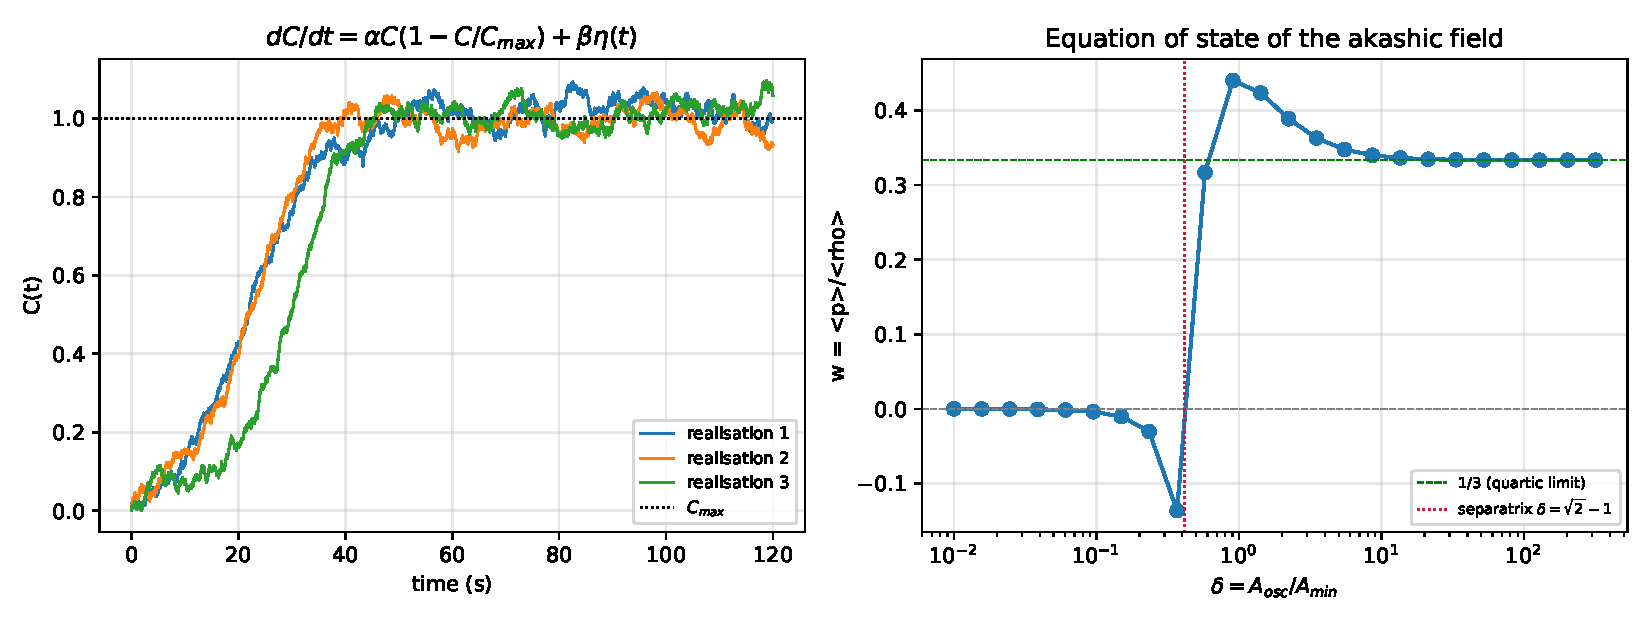
\includegraphics[width=0.95\textwidth]{figures/fig02_field_dynamics.pdf}
\caption{Links: drei Realisierungen des Bewusstseinsfeldes mit Rauschen, für $\alpha = 0,15$ s$^{-1}$ (Relaxationszeit 50 s). Rechts: die Zustandsgleichung $w(\delta)$ des Akasha-Feldes, exakt entlang der Bahn berechnet; die Separatrix liegt bei $\delta = \sqrt{2}-1$.}
\label{fig:camp}
\end{figure}

\section{Der neuronale Empfänger (Gehirn + Herz)}
